\section{EPW CSV Format (In/Out)}\label{epw-csv-format-inout}

EPW CSV Format to the Weather Converter is a special CSV format which echoes the format of the EPW file. For the ``header'' records in the CSV file, they are basically the same as the header records for the EPW file (see above). However, in the CSV file, each header is shown and then the data. Partial year files will not have all of these headers ``filled'' in. Also see Figure~\ref{fig:energyplus-epw-csv-file-spreadsheet-view}. EnergyPlus EPW CSV file (spreadsheet view) and Figure~\ref{fig:energyplus-epw-csv-data-records-spreadsheet}. EnergyPlus EPW CSV Data Records (spreadsheet view) for snapshot pictures of the EnergyPlus EPW CSV file as shown in a spreadsheet.

\subsection{Location Header/Data (CSV)}\label{location-headerdata-csv}

Location Title,Latitude \{N+/S-\},Longitude \{E+/W-\},TimeZone \{+/- GMT\},Elevation \{m\}

LOCATION\_SYDNEY\_\_AUS\_IWEC Data\_947670,-33.95,151.18,10.0,3.0

LOCATION + the city, state/province, country and WMO fields from the EPW file are concatenated to form the ``Location Title''. The latitude, longitude, time zone and elevation fields are numeric.

\subsection{Design Conditions Header/Data (CSV)}\label{design-conditions-headerdata-csv}

If there are design conditions, then the format is as follows:

Number of Design Conditions,Title of Design Condition,Design Stat,HDB 99.6\%,HDB 99\%,X WS 1\%,X WS 2.5\%,X WS 5\%,CM WS .4\%,CM MDB .4\%,CM WS 1\%,CM MDB 1\%,MWS 99.6\%,PWD 99.6\%,MWS .4\%,PWD .4\%,X MnDB Max,X MnDB Min,X StdDB Max,X StdDB Min,Design Stat,CDB .4\%,C MWB .4\%,CDB 1\%,C MWB 1\%,CDB 2\%,C MWB 2\%,E WB .4\%,E MDB .4\%,E WB 1\%,E MDB 1\%,E WB 2\%,E MDB 2\%,DP .4\%,HR .4\%,MDB .4\%,DP 1\%,HR 1\%,MDB 1\%,DP 2\%,HR 2\%,MDB 2\%,DB Range

,,Units,\{°C\},\{°C\},\{m/s\},\{m/s\},\{m/s\},\{m/s\},\{°C\},\{m/s\},\{°C\},\{m/s\},\{Degree\},\{m/s\},\{Degree\},\{°C\},\{°C\},\{°C\},\{°C\},Units,\{°C\},\{°C\},\{°C\},\{°C\},\{°C\},\{°C\},\{°C\},\{°C\},\{°C\},\{°C\},\{°C\},\{°C\},\{°C\},\{g/kg\},\{°C\},\{°C\},\{g/kg\},\{°C\},\{°C\},\{g/kg\},\{°C\},\{°C\}

1,World Climate Design Data 2001 ASHRAE Handbook,HEATING,5.8,6.8,11.3,9.9,8.8,11.1,14.2,9.1,13.4,1.1,320,5.3,300,39.3,3.1,2.9,1.9,COOLING,32.2,20,29.5,19.7,27.9,20.1,23,28,22.3,26.2,21.7,25.3,21.7,16.4,24.8,21.1,15.8,24.3,20.6,15.3,23.9,6.7

However, if there are no design conditions, then the format looks like:

Number of Design Conditions,Title of Design Condition,

0

Theoretically, there can be more than one design condition included.

\subsection{Typical/Extreme Periods Header/Data (CSV)}\label{typicalextreme-periods-headerdata-csv}

The results from the typical / extreme period heuristic calculation are shown.

Number of Typical/Extreme Periods,Period Name,Period Type,Period Start Day,Period End Day,\textless{}repeat to \# periods\textgreater{}

6,Summer - Week Nearest Max Temperature For Period,Extreme,1/ 4,1/10,Summer - Week Nearest Average Temperature For Period,Typical,11/29,12/ 5,Winter - Week Nearest Min Temperature For Period,Extreme,7/ 3,7/ 9,Winter - Week Nearest Average Temperature For Period,Typical,6/ 5,6/11,Autumn - Week Nearest Average Temperature For Period,Typical,3/22,3/28,Spring - Week Nearest Average Temperature For Period,Typical,8/ 1,8/ 7

\subsection{Ground Temperatures Header/Data (CSV)}\label{ground-temperatures-headerdata-csv}

The results from the ground temperature heuristic calculation are shown, typically for 3 depths. Users may also fill in the blank fields (soil conductivity, soil density, soil specific heat) with known values and/or perform their own calculations and depths and supply those. These should be considered ``undisturbed'' ground temperatures - temperatures of soil that have not been disturbed by construction. They are not considered appropriate for calculations of building losses.

The program uses a heuristic, time lagged calculation based on dry bulb temperature and location. References on the topic are found in Kusuda (see references).

Number of Ground Temperature Depths,Ground Temperature Depth \{m\},Soil Conductivity \{W/m-K\},Soil Density \{kg/m3\},Soil Specific Heat \{J/kg-K\},Jan \{C\},Feb\{C\},Mar \{C\},Apr \{C\},May \{C\},Jun \{C\},Jul \{C\},Aug \{C\},Sep \{C\},Oct \{C\},Nov \{C\},Dec \{C\},\textless{}repeat to Number of temperature depths\textgreater{}

3,.5,,,,20.69,22.30,22.69,22.26,19.95,17.43,15.09,13.43,12.99,13.86,15.84,18.29,2,,,,19.18,20.71,21.41,21.40,20.16,18.43,16.58,15.03,14.25,14.45,15.59,17.28,4,,,,18.18,19.38,20.10,20.30,19.82,18.80,17.56,16.35,15.56,15.39,15.89,16.89

\subsection{Holiday/Daylight Saving Header/Data (CSV)}\label{holidaydaylight-saving-headerdata-csv}

If these data are entered, the weather converter will process them. Default weather processing contains no holidays or daylight saving period. Of course, these can also be specified in your input data file for EnergyPlus and do not need to be embedded in the weather file.

Leap Year Observed?,Daylight Saving Start Date,Daylight Saving End Date,Number of Holidays,Holiday Name,Holiday Date,\textless{}repeat for \# Holidays\textgreater{}

No,0,0,0

\subsection{Comment 1 Header/Data (CSV)}\label{comment-1-headerdata-csv}

Some original data files fill the comment 1 header and some do not. Typically, it will display at least a ``station'' number and potentially more information.

Comment Line \#1

``IWEC- WMO\#947670 - South-west Pacific -- Original Source Data (c) 2001 American Society of Heating, Refrigerating and Air-Conditioning Engineers (ASHRAE), Inc., Atlanta, GA, USA. www.ashrae.org All rights reserved as noted in the License Agreement and Additional Conditions. DISCLAIMER OF WARRANTIES: The data is provided `as is' without warranty of any kind, either expressed or implied. The entire risk as to the quality and performance of the data is with you. In no event will ASHRAE or its contractors be liable to you for any damages, including without limitation any lost profits, lost savings, or other incidental or consequential damages arising out of the use or inability to use this data.''

\subsection{Comment 2 Header/Data (CSV)}\label{comment-2-headerdata-csv}

Comment Line \#2

-- Ground temps produced with a standard soil diffusivity of 2.3225760E-03 \{m**2/day\}

\subsection{Data Period Header/Data (CSV)}\label{data-period-headerdata-csv}

Number of Data Periods {[}DP{]},Number of Intervals per Hour,DP Name/Description,DP Start Day of Week,DP Start Day, DP End Day,\textless{}repeat to \# Data Periods\textgreater{}

1,1,Data,Sunday, 1/ 1,12/31

\subsection{Data Records (CSV)}\label{data-records-csv}

The field ``names'' for each item are shown. First, the ``short'' names:

Date,HH:MM,Datasource,DryBulb \{C\},DewPoint \{C\},RelHum \{\%\},Atmos Pressure \{Pa\},ExtHorzRad \{Wh/m2\},ExtDirRad \{Wh/m2\},HorzIRSky \{Wh/m2\},GloHorzRad \{Wh/m2\},DirNormRad \{Wh/m2\},DifHorzRad \{Wh/m2\},GloHorzIllum \{lux\},DirNormIllum \{lux\},DifHorzIllum \{lux\},ZenLum \{Cd/m2\},WindDir \{deg\},WindSpd \{m/s\},TotSkyCvr \{.1\},OpaqSkyCvr \{.1\},Visibility \{km\},Ceiling Hgt \{m\},PresWeathObs,PresWeathCodes,Precip Wtr \{mm\},Aerosol Opt Depth \{.001\},SnowDepth \{cm\},Days Last Snow,Albedo \{.01\},Rain \{mm\},Rain Quantity \{hr\}

Then, the longer names:

Date,HH:MM,Datasource,Dry Bulb Temperature \{C\},Dew Point Temperature \{C\},Relative Humidity \{\%\},Atmospheric Pressure \{Pa\},Extraterrestrial Horizontal Radiation \{Wh/m2\},Extraterrestrial Direct Normal Radiation \{Wh/m2\},Horizontal Infrared Radiation Intensity from Sky \{Wh/m2\},Global Horizontal Radiation \{Wh/m2\},Direct Normal Radiation \{Wh/m2\},Diffuse Horizontal Radiation \{Wh/m2\},Global Horizontal Illuminance \{lux\},Direct Normal Illuminance \{lux\},Diffuse Horizontal Illuminance \{lux\},Zenith Luminance \{Cd/m2\},Wind Direction \{deg\},Wind Speed \{m/s\},Total Sky Cover \{.1\},Opaque Sky Cover \{.1\},Visibility \{km\},Ceiling Height \{m\},Present Weather Observation,Present Weather Codes,Precipitable Water \{mm\},Aerosol Optical Depth \{.001\},Snow Depth \{cm\},Days Since Last Snow,Albedo \{.01\},Liquid Precipitation Depth \{mm\},Liquid Precipitation Quantity \{hr\}

As noted previously, these headers and data are in the identical order to the items in the EPW records. Then the data is shown:

1983/1/1,01:00,C9C9C9C9*0?9?9?9?9?9?9?9*0C8C8C8C8*0*0E8*0*0,26.2,19.2,65,101100,0,1415,412,0,0,0,0,0,0,0,180,6.5,9,7,23.3,77777,9,'999999999,0,0.2300,0,88

The Date and Time fields need a bit of description. The Date field (e.g.~1983/1/1) uses your standard system date for formatting. In the EPW file, these are three separate fields (year, month, and day in this example). The time field combines the hours and minutes into one field (hh:mm). This makes it easier for graphing with spreadsheet programs but a bit harder if you use the CSV format as input.

Each data item field obeys the same ``missing'' and other content rules as shown above in the EnergyPlus Weather File (EPW) Data Dictionary.

\begin{figure}[hbtp] % fig 17
\centering
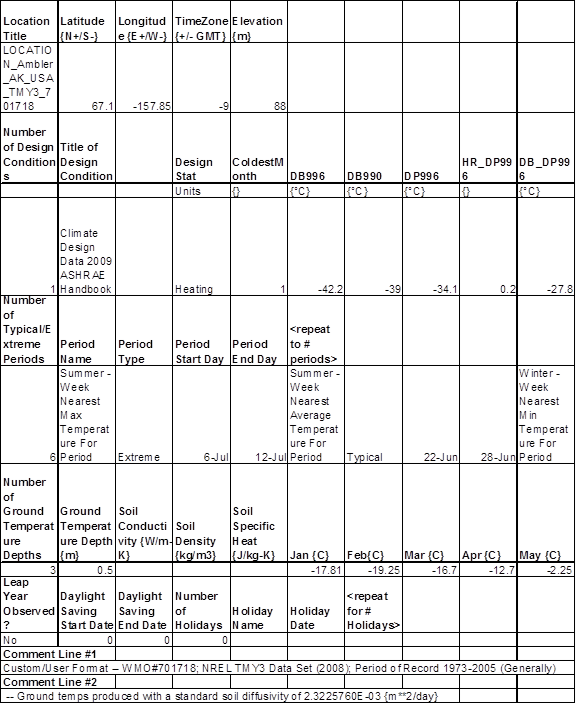
\includegraphics[width=0.9\textwidth, height=0.9\textheight, keepaspectratio=true]{media/image015.png}
\caption{EnergyPlus EPW CSV file (spreadsheet view) \protect \label{fig:energyplus-epw-csv-file-spreadsheet-view}}
\end{figure}

The figure above shows how the EnergyPlus EPW CSV file (initial header records) looks when opened in a spreadsheet. Each header record is shown in bold with data following the headers..

\begin{figure}[hbtp] % fig 18
\centering
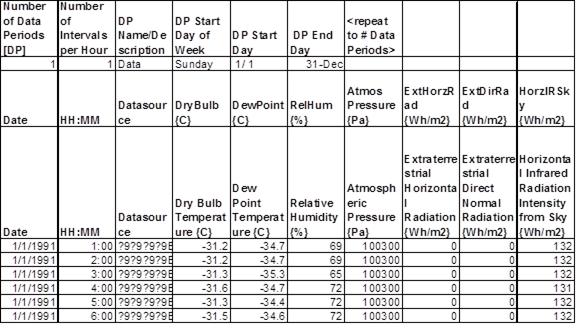
\includegraphics[width=0.9\textwidth, height=0.9\textheight, keepaspectratio=true]{media/image016.png}
\caption{EnergyPlus EPW CSV Data Records (spreadsheet view) \protect \label{fig:energyplus-epw-csv-data-records-spreadsheet}}
\end{figure}

The above figure shows how the data periods header record and the individual data records look when opened in a spread sheet. Again, the headers are shown in bold. Note that there are two header records for the data records - one with short names - one with longer more descriptive names.
